\documentclass[11pt,a4paper]{article}
\usepackage[margin=2.2cm]{geometry}
\usepackage{graphicx}
\usepackage{booktabs}
\usepackage{amsmath}
\usepackage[colorlinks=true,linkcolor=black,urlcolor=blue!60!black]{hyperref}
\usepackage{parskip}
\usepackage{caption}
\usepackage{pdflscape}
\captionsetup{font=small,labelfont=bf}

\title{\vspace{-1.6cm}Who wins a hash collision?\\[2pt]
\large A measurement of the collision argument in instant-NGP}
\author{\small measured by \texttt{scripts/collision\_audit.py} in \texttt{ngp-demo}}
\date{\small\today}

\begin{document}
\maketitle
\vspace{-0.8cm}

\section*{The claim under test}

M\"uller et al.\ (2022), \S3, explain why a hash table with no collision handling
still reconstructs a scene faithfully:

\begin{quote}\small
``When training samples collide in this way, their gradients average. Consider
that the importance to the final reconstruction of such samples is rarely equal.
\dots As a result, the gradients of the more important samples dominate the
collision average and the aliased table entry will naturally be optimized in such
a way that it reflects the needs of the higher-weighted point.''
\end{quote}

Two distant points that hash to the same row do not overwrite one another. The row
is one parameter receiving the \emph{sum} of two pulls, and it settles where the
stronger pull wants it. In a radiance field ``stronger'' means density $\times$
visibility. The question this note answers is whether that story survives being
measured, and how much the loser actually pays.

\section*{The design, and why it is not circular}

The tempting experiment --- fit a painting and observe that the detailed parts come
out sharper than the flat parts --- proves nothing. Detailed regions are sampled
against more structure, occupy different levels and hold different amounts of
error, so any asymmetry has half a dozen possible causes.

So importance is made an explicit knob and everything else is held fixed:

\begin{itemize}\itemsep2pt
\item The painting is cut into a \textbf{checkerboard of \CHKBLOCK{} px blocks}. Region A
is the bright squares of panel (a), region B the dimmed ones. They are the same
picture at the same scales, interleaved: \PXA{} against \PXB{} pixels, mean
$|\nabla I|$ \DETA{} against \DETB{}. Panel (b) confirms the consequence that
matters --- on every hashed level the two regions put the \emph{same}
interpolation weight on the rows they share, within \WEIGHTDEV{}.
\item Region B is fitted at \textbf{loss weight $\lambda$}; region A always at 1.
This is the paper's ``importance'', made a dial: $\lambda$ multiplies exactly the
gradient B delivers, and nothing else.
\item Each $\lambda$ is run \textbf{twice}: once with a table small enough that the
fine levels collide ($T=2^{\SMALLT}$, \HASHEDLEVELS{} of \NLEVELS{} levels hashed) and
once with a table large enough that \textbf{every} level is dense ($T=2^{\LARGET}$,
0 hashed). The dense run is the control that separates \emph{B learns less because
its gradients are small} from \emph{B loses its shared rows to A}.
\end{itemize}

The encoder is the one \texttt{scripts/gui\_image.py} fits by default (L\,=\,\NLEVELS,
F\,=\,2, coarsest 4 cells, $b$\,=\,1.35, finest capped at the pixel count), on the
painting at \IMSIZE, \STEPS{} steps of Adam at lr \LR{} with batch \BATCH.

% Landscape, on its own page: the figure is 16.5 x 9.4 in and unreadable at
% portrait \textwidth.
\begin{landscape}
\begin{figure}[p]
\centering
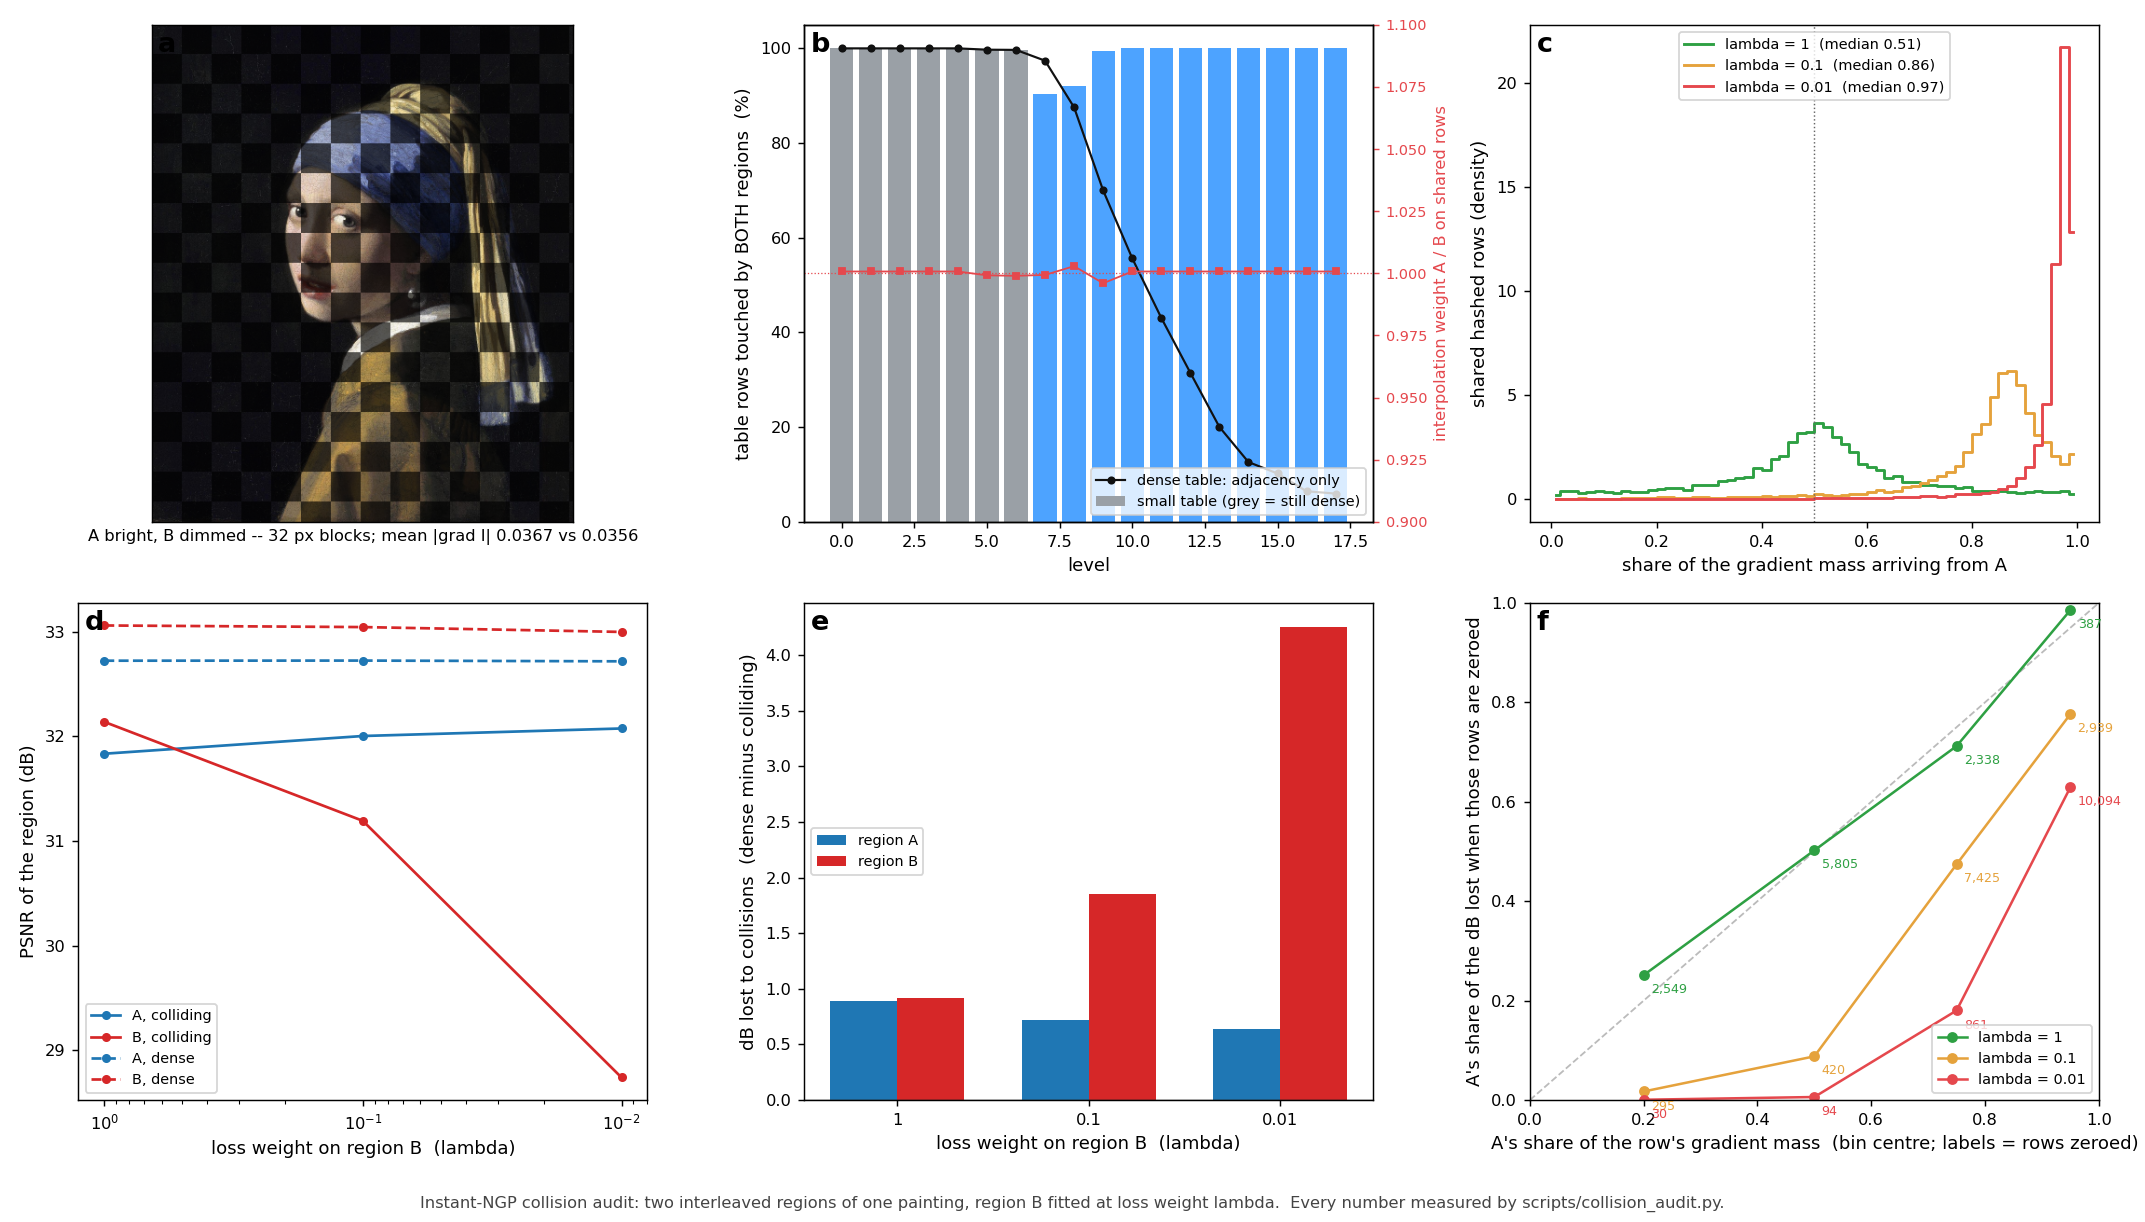
\includegraphics[width=\linewidth]{../figures/collision_audit.png}
\caption{The audit. \textbf{(a)} the two regions. \textbf{(b)} how the two regions
come to share a table row, level by level: the black line is the dense table, where
sharing can only mean adjacency, and it falls to \DENSESHAREFINE{}\% at the finest
level; the bars are the small table, where sharing is \SMALLSHAREFINE{}\%. The red
squares are the balance check. \textbf{(c)} where a shared row's gradient mass comes
from, one histogram per $\lambda$. \textbf{(d)} the outcome: solid = colliding,
dashed = dense. \textbf{(e)} the same, as what each region lost to collisions.
\textbf{(f)} zeroing shared rows, grouped by A's share of their gradient mass; the
dashed diagonal is ``damage in proportion to mass''.}
\end{figure}
\end{landscape}

\section*{What was measured}

\begin{table}[h]\centering\small
\begin{tabular}{lccccc}
\toprule
& \multicolumn{2}{c}{colliding, $T=2^{\SMALLT}$} & \multicolumn{2}{c}{dense, $T=2^{\LARGET}$} & \\
\cmidrule(lr){2-3}\cmidrule(lr){4-5}
$\lambda$ & A (dB) & B (dB) & A (dB) & B (dB) & B's loss to collisions \\
\midrule
\RUNROWS
\bottomrule
\end{tabular}
\caption{Per-region PSNR. \NENTSMALL{} table rows against \NENTDENSE{}.}
\end{table}

\textbf{1. Equal weights, equal outcome.} At $\lambda=1$ the two regions land
\LAMONEGAP{} dB apart with collisions and \LAMONEGAPD{} dB apart without, and
collisions cost them \LAMONECOSTA{} and \LAMONECOSTB{} dB respectively. The
checkerboard is fair, and a shared table is not by itself unfair.

\textbf{2. Weight alone costs nothing.} Down-weighting B by $100\times$ in the
\emph{dense} table moves it by \DENSEDRIFT{} dB (\DENSEBONE{} $\to$ \DENSEBHUN{}).
With its own rows, a region fitted at $\lambda=0.01$ is fitted just as well; the
gradients are smaller but they point the same way, and Adam is scale-free per
parameter. This is the control that makes the next line mean something.

\textbf{3. Weight decides who owns a shared row.} The gradient mass arriving at a
shared hashed row is split \DOMONE{} in favour of A at $\lambda=1$ (median over
\NSHARED{} rows) --- the checkerboard's balance, showing up in the training signal.
At $\lambda=0.1$ that median is \DOMTEN, at $\lambda=0.01$ it is \DOMHUN, with
\DOMHUNFRAC{}\% of shared rows above 0.9. Panel (c) is the collision average
tilting, exactly as \S3 describes.

\textbf{4. And the loser pays, in dB.} At $\lambda=0.01$, B loses \COSTBHUN{} dB to
collisions while A loses \COSTAHUN{} --- \COSTRATIO{} times as much, for a region
that touches those rows equally often. Panel (e): what B pays grows \COSTBONE{}
$\to$ \COSTBTEN{} $\to$ \COSTBHUN{} dB as its weight falls, while A's cost
\emph{shrinks} \COSTAONE{} $\to$ \COSTATEN{} $\to$ \COSTAHUN{}. The shared capacity
is not destroyed by the collision; it is transferred.

\textbf{5. The transfer is legible row by row.} Panel (f) zeroes shared rows grouped
by A's share of their gradient mass and asks who notices. At $\lambda=1$ the answer
tracks the diagonal: the 0--0.4 bin (\PFONELOWN{} rows, mass mostly from B) hands A
only \PFONELOW{} of the damage, and the 0.9--1 bin (\PFONEHIGHN{} rows) hands A
\PFONEHIGH{}. At equal loss weights nothing imposed that split --- it is what the
residuals happened to do --- and it still predicts, row by row, whose picture the
row is holding.

\section*{What this does not show}

\begin{itemize}\itemsep2pt
\item \textbf{The loser is not unharmed, and A is not unharmed either.} At
$\lambda=0.01$ the dominant bin holds \PFHUNHIGHN{} rows and zeroing them still costs
B \PFHUNHIGHB{} dB. Panel (f) sits \emph{below} the diagonal at low $\lambda$: B
reads those rows constantly, it just no longer sets them. ``Reflects the needs of
the higher-weighted point'' is a statement about where the row settles, not a claim
that the other point stopped depending on it.
\item \textbf{Importance here is a loss weight}, imposed from outside. In a radiance
field it is density $\times$ visibility, which the fit itself produces and which
therefore co-evolves with the table. That feedback is not present in this test.
\item \textbf{This is a 2D image under an L2 loss with uniform sampling.} The
sampling density of the two regions is equal by construction; a task whose samples
concentrate somewhere --- the paper's ``online adaptivity'' --- is a different
measurement.
\item \textbf{The dense control has \NENTDENSE{} rows against \NENTSMALL{}}, so its
absolute PSNR is not comparable with the colliding runs. Every claim above is
either a within-run A-versus-B comparison or a same-region difference across the two
tables, both of which are unaffected.
\end{itemize}

\section*{Reproduce}

\begin{verbatim}
python scripts/collision_audit.py                 # 6 fits, writes the png and the json
python scripts/collision_audit.py --replot        # rebuild the figure from the json
\end{verbatim}

Every number in this note is read from \texttt{figures/collision\_audit.json}, and
this note is generated by \texttt{note/build\_note.py} from that file.

\end{document}
